\chapter{Background and Literature Review}\label{ch:problem}
%---------------------------------------------------------
\section{Preliminaries and Notation}\label{preliminaries}
This thesis uses the following notation, nomenclature, and fundamental equations of motion for fixed wing rigid body aerodynamics.

\subsection{Kinematics}
The following is the nomenclature that will be used to describe the kinematic equations.  Euler angles for pitch $(\theta)$, roll $(\phi)$, and yaw $(\psi)$ will have the units of radians.  The following Figure~\ref{fig:reference_frame} illustrates the \ac{NED} reference frame definitions used for body rotational rates about the $x$ axis $(p)$, $y$ axis $(q)$, and the $z$ axis $(r)$ as well as the body velocities in the $x$ axis $(u)$, $y$ axis $(v)$, and the $z$ axis $(w)$.

\begin{figure}[h!]
 \centering
  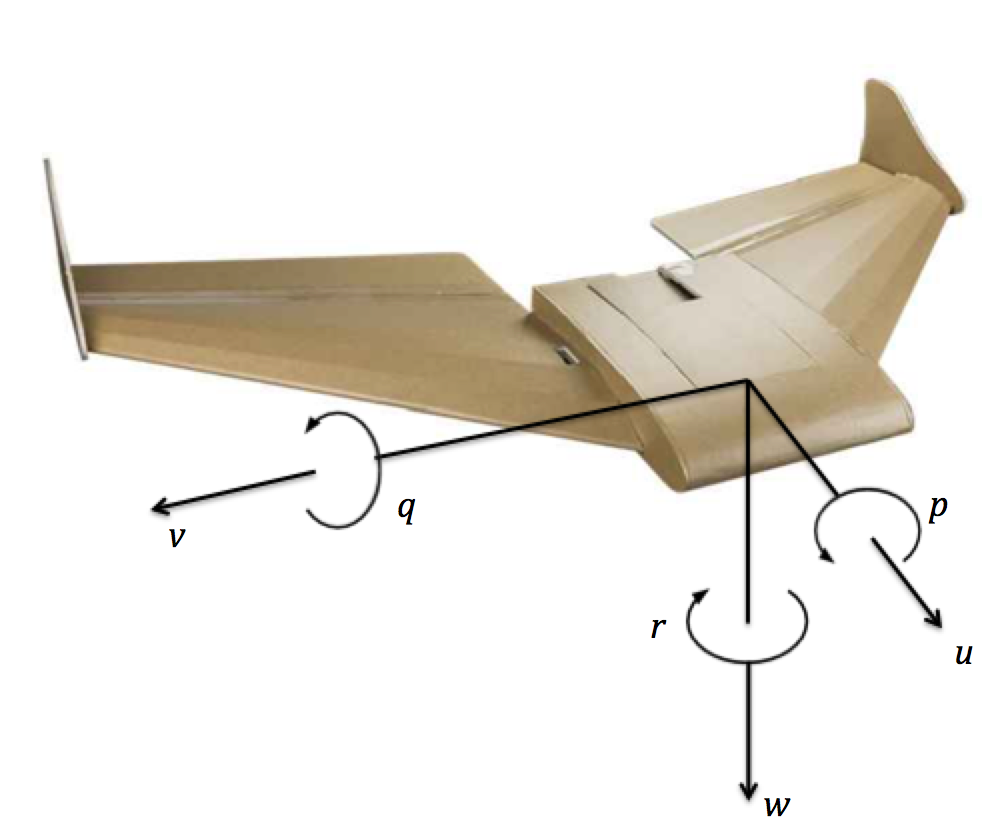
\includegraphics[width=0.65\textwidth]{body_frame_rotations.png}
  \caption{Reference frame - body rates and velocities}
  \label{fig:reference_frame}
\end{figure}

\subsection{First Order Model}
The following nomenclature will be used to illustrate the modeling of first order systems where $\dot{x}$ is the time derivative of the state, A is the Hurwitz matrix, B is the input matrix, and u is the input vector.
\begin{equation}
\dot{x}(t)=Ax(t)+Bu(t)
\end{equation}

\subsection{Second Order Model}


%---------------------------------------------------------
\section{Feedback vs Adaptive Control}

\begin{figure}[h!]
 \centering
  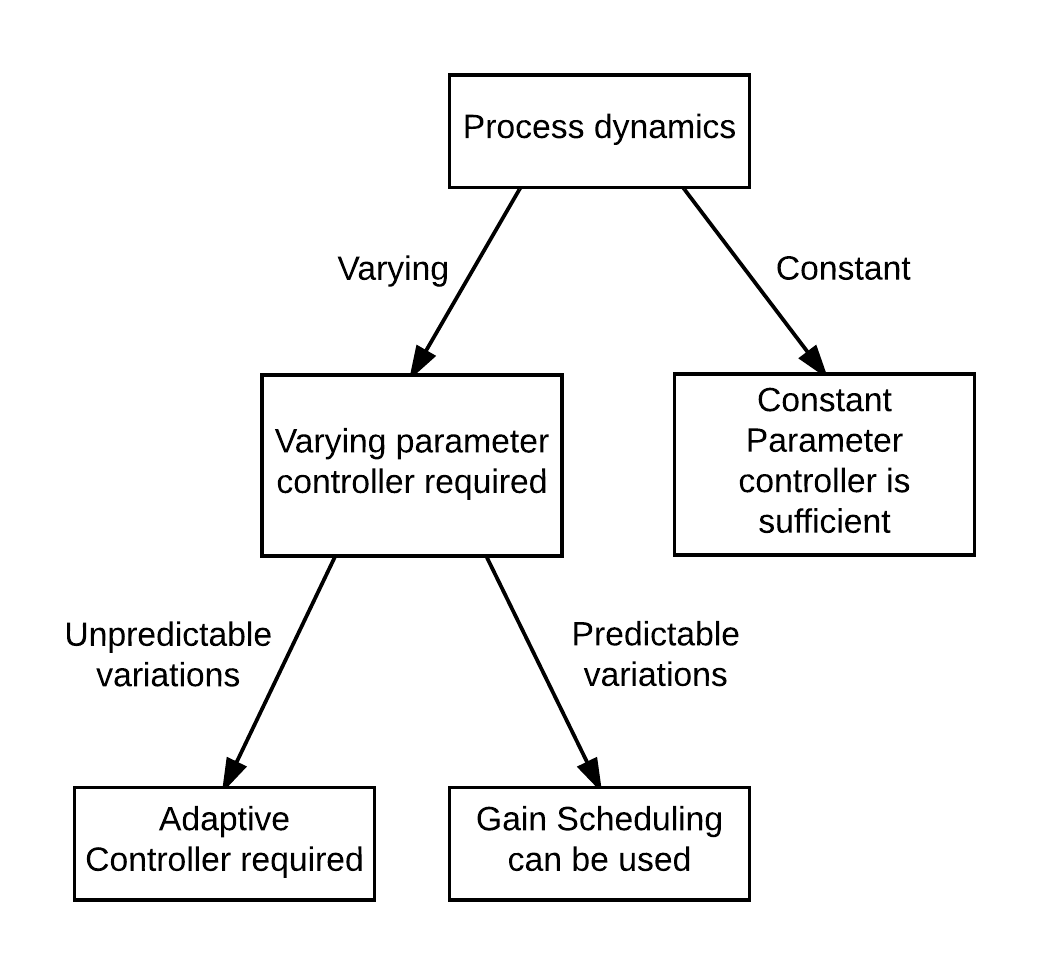
\includegraphics[width=0.85\textwidth]{why_adaptive_control.png}
  \caption{Determine if adaptive control should be used}
  \label{fig:why_adaptive_control}
\end{figure}


%---------------------------------------------------------
\section{MIT Rule}


%---------------------------------------------------------
\section{Lyapunov Stability Criteria}

Aerospace controllers tend to use linear controllers for their simplicity and well understood robustness characteristics.  This is despite the fact that the applications of these linear controllers are applied to non-linear control solutions such as attitude control with varying dynamic pressure.  Adaptive Controllers are non-linear and may offer performance benefits to non-linear systems as seen in aerospace applications.  However, non-linear controller's robustness properties need to be evaluated.  The Lyapunov stability criteria offers methods of evaluating these controller's boundedness and robustness behavior.  

Lyapunov was a Russian mathematician who's work was published in 1892 concerning the behavior of non-linear systems around equilibrium without having to find the unique solutions to often difficult differential equations used to model the system.  His work was largely overlooked until the Cold War when aerospace solutions required a more rigorous approach to analyzing non-linear control robustness.  Modern non-linear control engineers exclusively utilize Lyapunov's techniques to design non-linear controllers and evaluate their contributions to non-linear dynamical systems.

\subsection{Lyapunov's Second Method}
 


